% The default tree with its contour (top) and the birth-exchanged tree with the
% time-reversed contour (bottom). Coordinates follow fig:cont-right-bdp and fig:cont-left-bdp of
% Paper01_AgeBDPVarEnv/sections/4_Contours.tex.
% Compile with: pdflatex "\def\stage{k}% The default tree with its contour (top) and the birth-exchanged tree with the
% time-reversed contour (bottom). Coordinates follow fig:cont-right-bdp and fig:cont-left-bdp of
% Paper01_AgeBDPVarEnv/sections/4_Contours.tex.
% Compile with: pdflatex "\def\stage{k}% The default tree with its contour (top) and the birth-exchanged tree with the
% time-reversed contour (bottom). Coordinates follow fig:cont-right-bdp and fig:cont-left-bdp of
% Paper01_AgeBDPVarEnv/sections/4_Contours.tex.
% Compile with: pdflatex "\def\stage{k}% The default tree with its contour (top) and the birth-exchanged tree with the
% time-reversed contour (bottom). Coordinates follow fig:cont-right-bdp and fig:cont-left-bdp of
% Paper01_AgeBDPVarEnv/sections/4_Contours.tex.
% Compile with: pdflatex "\def\stage{k}\input{exchanged_pair.tex}"   (k = 1..2)
%   1 both pictures      2 first ascent (top) and last descent (bottom) highlighted;
%                        they are the same path run in opposite directions
\documentclass[tikz,border=4pt]{standalone}
\usepackage{xcolor}
\usepackage{libertinus-otf}
\usepackage{unicode-math}
\setmathfont{STIX Two Math}
\definecolor{paper}{HTML}{FAFAFA}
\definecolor{treecol}{HTML}{D55E00}
\definecolor{contcol}{HTML}{0072B2}

\ifcase\stage\or
  \def\hiop{1}\def\loop{1}\def\treeop{1}\or
  \def\hiop{1}\def\loop{0.15}\def\treeop{0.35}\fi

\begin{document}
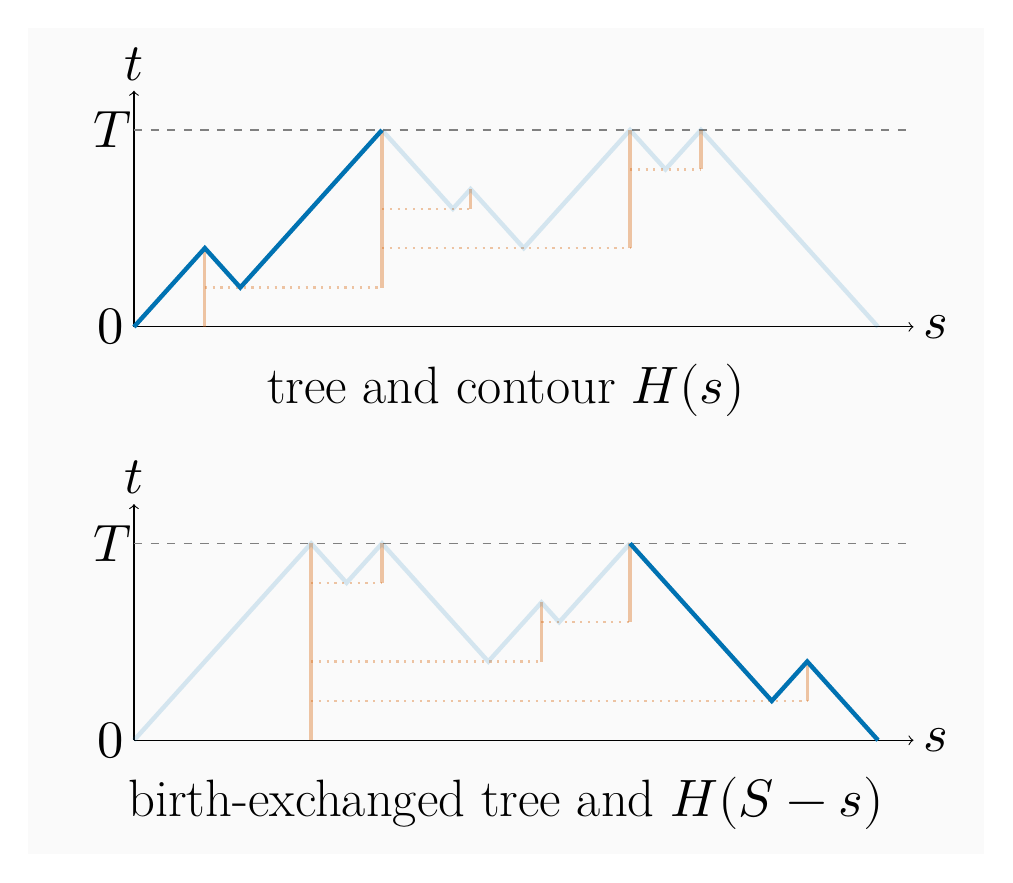
\begin{tikzpicture}[xscale=0.45, yscale=0.5, font=\fontsize{19pt}{23pt}\selectfont]
  \fill[paper] (-3,-13.4) rectangle (24,7.6);

  % ---- Top: the default tree and its contour H(s) ------------------------------------
  \begin{scope}
    \draw[->] (0,0) -- (22,0) node[right] {$s$};
    \draw[->] (0,0) -- (0,6) node[above] {$t$};
    \draw[dashed, gray] (0,5) -- (22,5);
    \node[left] at (0,5) {$T$};
    \node[left] at (0,0) {$0$};

    \draw[very thick, treecol, opacity=\treeop]
      (2,0) -- (2,2) (7,1) -- (7,5) (14,2) -- (14,5) (9.5,3) -- (9.5,3.5) (16,4) -- (16,5);
    \draw[thick, treecol, dotted, opacity=\treeop]
      (2,1) -- (7,1) (7,2) -- (14,2) (7,3) -- (9.5,3) (14,4) -- (16,4);

    \draw[ultra thick, contcol, opacity=\hiop] (0,0) -- (2,2) -- (3,1) -- (7,5);
    \draw[ultra thick, contcol, opacity=\loop]
      (7,5) -- (9,3) -- (9.5,3.5) -- (11,2) -- (14,5) -- (15,4) -- (16,5) -- (21,0);

    \node at (10.5,-1.6) {tree and contour $H(s)$};
  \end{scope}

  % ---- Bottom: the birth-exchanged tree, contour H(S - s) ---------------------------------
  \begin{scope}[shift={(0,-10.5)}]
    \draw[->] (0,0) -- (22,0) node[right] {$s$};
    \draw[->] (0,0) -- (0,6) node[above] {$t$};
    \draw[dashed, gray] (0,5) -- (22,5);
    \node[left] at (0,5) {$T$};
    \node[left] at (0,0) {$0$};

    \draw[very thick, treecol, opacity=\treeop]
      (5,0) -- (5,5) (7,4) -- (7,5) (11.5,2) -- (11.5,3.5) (14,3) -- (14,5) (19,1) -- (19,2);
    \draw[thick, treecol, dotted, opacity=\treeop]
      (5,4) -- (7,4) (5,2) -- (11.5,2) (11.5,3) -- (14,3) (5,1) -- (19,1);

    \draw[ultra thick, contcol, opacity=\loop]
      (0,0) -- (5,5) -- (6,4) -- (7,5) -- (10,2) -- (11.5,3.5) -- (12,3) -- (14,5);
    \draw[ultra thick, contcol, opacity=\hiop] (14,5) -- (18,1) -- (19,2) -- (21,0);

    \node at (10.5,-1.6) {birth-exchanged tree and $H(S-s)$};
  \end{scope}
\end{tikzpicture}
\end{document}
"   (k = 1..2)
%   1 both pictures      2 first ascent (top) and last descent (bottom) highlighted;
%                        they are the same path run in opposite directions
\documentclass[tikz,border=4pt]{standalone}
\usepackage{xcolor}
\usepackage{libertinus-otf}
\usepackage{unicode-math}
\setmathfont{STIX Two Math}
\definecolor{paper}{HTML}{FAFAFA}
\definecolor{treecol}{HTML}{D55E00}
\definecolor{contcol}{HTML}{0072B2}

\ifcase\stage\or
  \def\hiop{1}\def\loop{1}\def\treeop{1}\or
  \def\hiop{1}\def\loop{0.15}\def\treeop{0.35}\fi

\begin{document}
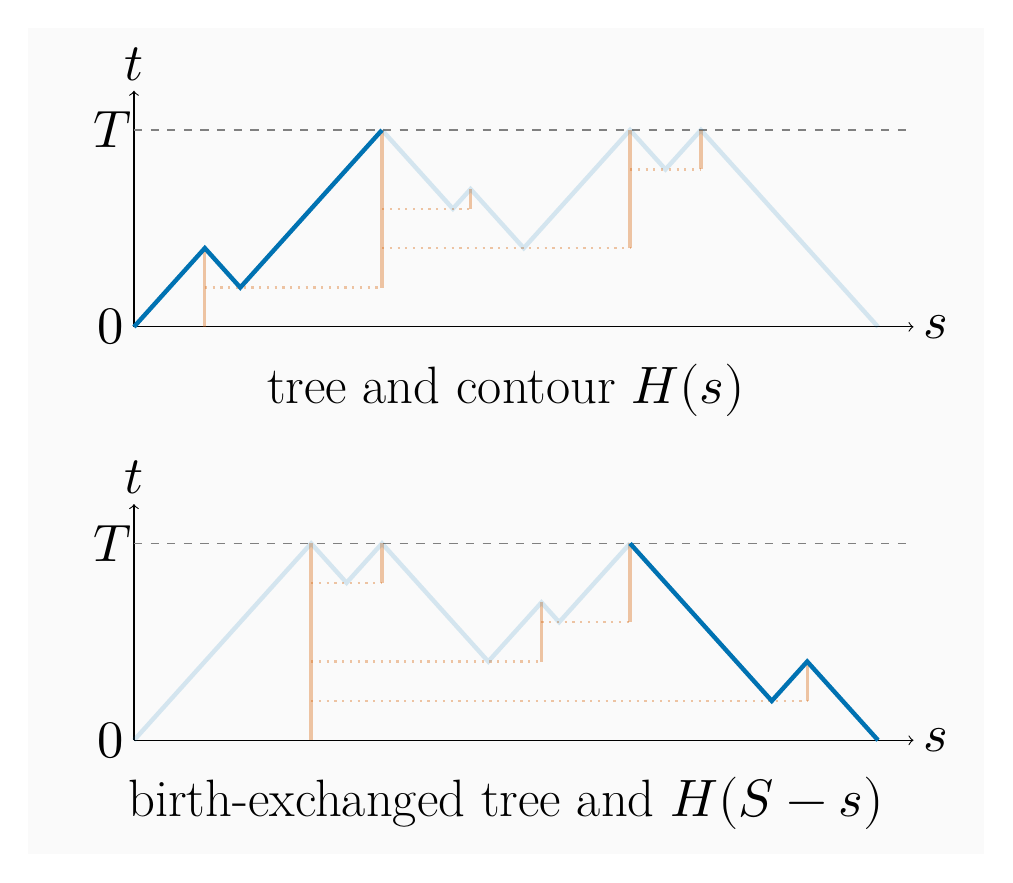
\begin{tikzpicture}[xscale=0.45, yscale=0.5, font=\fontsize{19pt}{23pt}\selectfont]
  \fill[paper] (-3,-13.4) rectangle (24,7.6);

  % ---- Top: the default tree and its contour H(s) ------------------------------------
  \begin{scope}
    \draw[->] (0,0) -- (22,0) node[right] {$s$};
    \draw[->] (0,0) -- (0,6) node[above] {$t$};
    \draw[dashed, gray] (0,5) -- (22,5);
    \node[left] at (0,5) {$T$};
    \node[left] at (0,0) {$0$};

    \draw[very thick, treecol, opacity=\treeop]
      (2,0) -- (2,2) (7,1) -- (7,5) (14,2) -- (14,5) (9.5,3) -- (9.5,3.5) (16,4) -- (16,5);
    \draw[thick, treecol, dotted, opacity=\treeop]
      (2,1) -- (7,1) (7,2) -- (14,2) (7,3) -- (9.5,3) (14,4) -- (16,4);

    \draw[ultra thick, contcol, opacity=\hiop] (0,0) -- (2,2) -- (3,1) -- (7,5);
    \draw[ultra thick, contcol, opacity=\loop]
      (7,5) -- (9,3) -- (9.5,3.5) -- (11,2) -- (14,5) -- (15,4) -- (16,5) -- (21,0);

    \node at (10.5,-1.6) {tree and contour $H(s)$};
  \end{scope}

  % ---- Bottom: the birth-exchanged tree, contour H(S - s) ---------------------------------
  \begin{scope}[shift={(0,-10.5)}]
    \draw[->] (0,0) -- (22,0) node[right] {$s$};
    \draw[->] (0,0) -- (0,6) node[above] {$t$};
    \draw[dashed, gray] (0,5) -- (22,5);
    \node[left] at (0,5) {$T$};
    \node[left] at (0,0) {$0$};

    \draw[very thick, treecol, opacity=\treeop]
      (5,0) -- (5,5) (7,4) -- (7,5) (11.5,2) -- (11.5,3.5) (14,3) -- (14,5) (19,1) -- (19,2);
    \draw[thick, treecol, dotted, opacity=\treeop]
      (5,4) -- (7,4) (5,2) -- (11.5,2) (11.5,3) -- (14,3) (5,1) -- (19,1);

    \draw[ultra thick, contcol, opacity=\loop]
      (0,0) -- (5,5) -- (6,4) -- (7,5) -- (10,2) -- (11.5,3.5) -- (12,3) -- (14,5);
    \draw[ultra thick, contcol, opacity=\hiop] (14,5) -- (18,1) -- (19,2) -- (21,0);

    \node at (10.5,-1.6) {birth-exchanged tree and $H(S-s)$};
  \end{scope}
\end{tikzpicture}
\end{document}
"   (k = 1..2)
%   1 both pictures      2 first ascent (top) and last descent (bottom) highlighted;
%                        they are the same path run in opposite directions
\documentclass[tikz,border=4pt]{standalone}
\usepackage{xcolor}
\usepackage{libertinus-otf}
\usepackage{unicode-math}
\setmathfont{STIX Two Math}
\definecolor{paper}{HTML}{FAFAFA}
\definecolor{treecol}{HTML}{D55E00}
\definecolor{contcol}{HTML}{0072B2}

\ifcase\stage\or
  \def\hiop{1}\def\loop{1}\def\treeop{1}\or
  \def\hiop{1}\def\loop{0.15}\def\treeop{0.35}\fi

\begin{document}
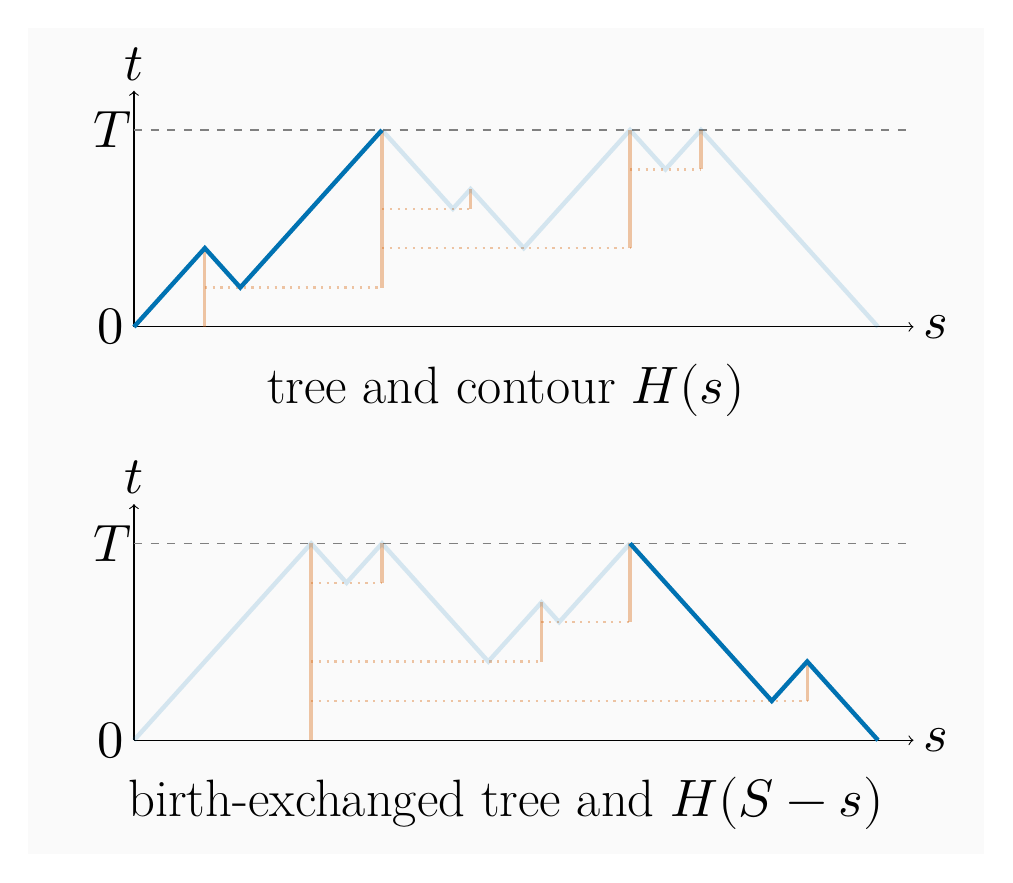
\begin{tikzpicture}[xscale=0.45, yscale=0.5, font=\fontsize{19pt}{23pt}\selectfont]
  \fill[paper] (-3,-13.4) rectangle (24,7.6);

  % ---- Top: the default tree and its contour H(s) ------------------------------------
  \begin{scope}
    \draw[->] (0,0) -- (22,0) node[right] {$s$};
    \draw[->] (0,0) -- (0,6) node[above] {$t$};
    \draw[dashed, gray] (0,5) -- (22,5);
    \node[left] at (0,5) {$T$};
    \node[left] at (0,0) {$0$};

    \draw[very thick, treecol, opacity=\treeop]
      (2,0) -- (2,2) (7,1) -- (7,5) (14,2) -- (14,5) (9.5,3) -- (9.5,3.5) (16,4) -- (16,5);
    \draw[thick, treecol, dotted, opacity=\treeop]
      (2,1) -- (7,1) (7,2) -- (14,2) (7,3) -- (9.5,3) (14,4) -- (16,4);

    \draw[ultra thick, contcol, opacity=\hiop] (0,0) -- (2,2) -- (3,1) -- (7,5);
    \draw[ultra thick, contcol, opacity=\loop]
      (7,5) -- (9,3) -- (9.5,3.5) -- (11,2) -- (14,5) -- (15,4) -- (16,5) -- (21,0);

    \node at (10.5,-1.6) {tree and contour $H(s)$};
  \end{scope}

  % ---- Bottom: the birth-exchanged tree, contour H(S - s) ---------------------------------
  \begin{scope}[shift={(0,-10.5)}]
    \draw[->] (0,0) -- (22,0) node[right] {$s$};
    \draw[->] (0,0) -- (0,6) node[above] {$t$};
    \draw[dashed, gray] (0,5) -- (22,5);
    \node[left] at (0,5) {$T$};
    \node[left] at (0,0) {$0$};

    \draw[very thick, treecol, opacity=\treeop]
      (5,0) -- (5,5) (7,4) -- (7,5) (11.5,2) -- (11.5,3.5) (14,3) -- (14,5) (19,1) -- (19,2);
    \draw[thick, treecol, dotted, opacity=\treeop]
      (5,4) -- (7,4) (5,2) -- (11.5,2) (11.5,3) -- (14,3) (5,1) -- (19,1);

    \draw[ultra thick, contcol, opacity=\loop]
      (0,0) -- (5,5) -- (6,4) -- (7,5) -- (10,2) -- (11.5,3.5) -- (12,3) -- (14,5);
    \draw[ultra thick, contcol, opacity=\hiop] (14,5) -- (18,1) -- (19,2) -- (21,0);

    \node at (10.5,-1.6) {birth-exchanged tree and $H(S-s)$};
  \end{scope}
\end{tikzpicture}
\end{document}
"   (k = 1..2)
%   1 both pictures      2 first ascent (top) and last descent (bottom) highlighted;
%                        they are the same path run in opposite directions
\documentclass[tikz,border=4pt]{standalone}
\usepackage{xcolor}
\usepackage{libertinus-otf}
\usepackage{unicode-math}
\setmathfont{STIX Two Math}
\definecolor{paper}{HTML}{FAFAFA}
\definecolor{treecol}{HTML}{D55E00}
\definecolor{contcol}{HTML}{0072B2}

\ifcase\stage\or
  \def\hiop{1}\def\loop{1}\def\treeop{1}\or
  \def\hiop{1}\def\loop{0.15}\def\treeop{0.35}\fi

\begin{document}
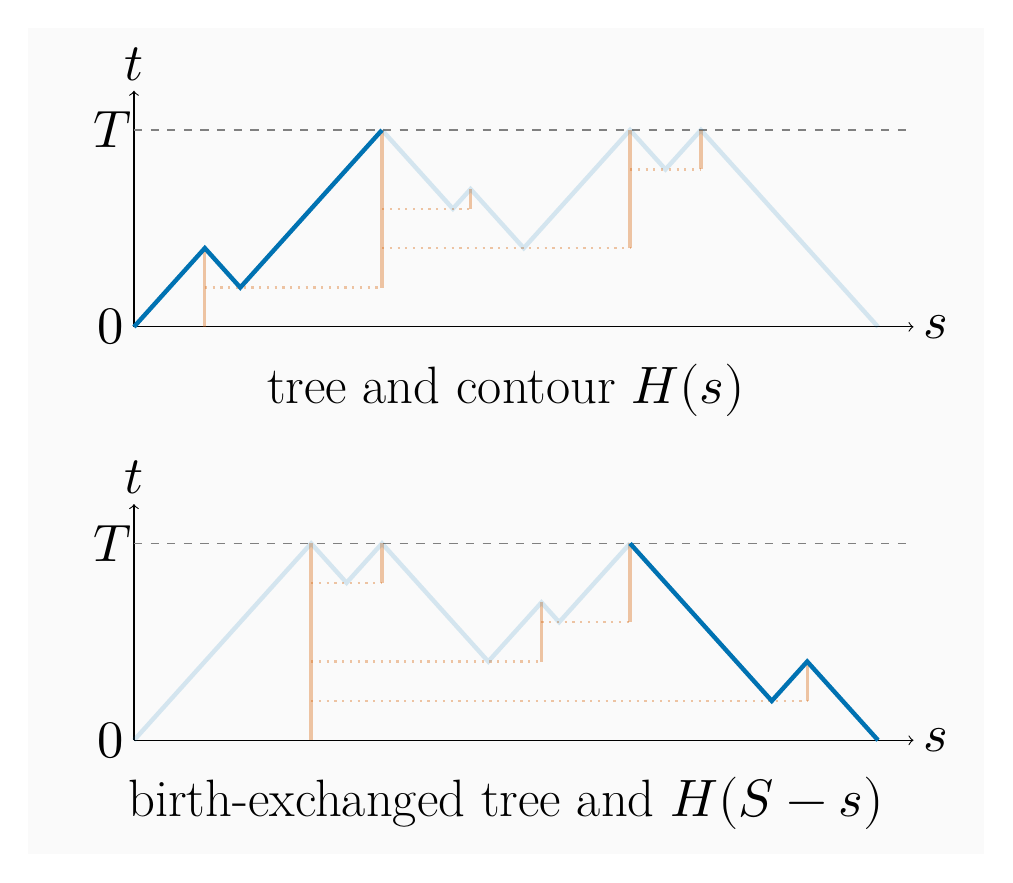
\begin{tikzpicture}[xscale=0.45, yscale=0.5, font=\fontsize{19pt}{23pt}\selectfont]
  \fill[paper] (-3,-13.4) rectangle (24,7.6);

  % ---- Top: the default tree and its contour H(s) ------------------------------------
  \begin{scope}
    \draw[->] (0,0) -- (22,0) node[right] {$s$};
    \draw[->] (0,0) -- (0,6) node[above] {$t$};
    \draw[dashed, gray] (0,5) -- (22,5);
    \node[left] at (0,5) {$T$};
    \node[left] at (0,0) {$0$};

    \draw[very thick, treecol, opacity=\treeop]
      (2,0) -- (2,2) (7,1) -- (7,5) (14,2) -- (14,5) (9.5,3) -- (9.5,3.5) (16,4) -- (16,5);
    \draw[thick, treecol, dotted, opacity=\treeop]
      (2,1) -- (7,1) (7,2) -- (14,2) (7,3) -- (9.5,3) (14,4) -- (16,4);

    \draw[ultra thick, contcol, opacity=\hiop] (0,0) -- (2,2) -- (3,1) -- (7,5);
    \draw[ultra thick, contcol, opacity=\loop]
      (7,5) -- (9,3) -- (9.5,3.5) -- (11,2) -- (14,5) -- (15,4) -- (16,5) -- (21,0);

    \node at (10.5,-1.6) {tree and contour $H(s)$};
  \end{scope}

  % ---- Bottom: the birth-exchanged tree, contour H(S - s) ---------------------------------
  \begin{scope}[shift={(0,-10.5)}]
    \draw[->] (0,0) -- (22,0) node[right] {$s$};
    \draw[->] (0,0) -- (0,6) node[above] {$t$};
    \draw[dashed, gray] (0,5) -- (22,5);
    \node[left] at (0,5) {$T$};
    \node[left] at (0,0) {$0$};

    \draw[very thick, treecol, opacity=\treeop]
      (5,0) -- (5,5) (7,4) -- (7,5) (11.5,2) -- (11.5,3.5) (14,3) -- (14,5) (19,1) -- (19,2);
    \draw[thick, treecol, dotted, opacity=\treeop]
      (5,4) -- (7,4) (5,2) -- (11.5,2) (11.5,3) -- (14,3) (5,1) -- (19,1);

    \draw[ultra thick, contcol, opacity=\loop]
      (0,0) -- (5,5) -- (6,4) -- (7,5) -- (10,2) -- (11.5,3.5) -- (12,3) -- (14,5);
    \draw[ultra thick, contcol, opacity=\hiop] (14,5) -- (18,1) -- (19,2) -- (21,0);

    \node at (10.5,-1.6) {birth-exchanged tree and $H(S-s)$};
  \end{scope}
\end{tikzpicture}
\end{document}
